\documentclass{beamer}

% Theme setting
\usetheme{Madrid} % This theme is quite flexible and popular

\usepackage{graphicx} % Required for including images
\usepackage{caption} % Required for captioning

\hypersetup{
    colorlinks=true,
    linkcolor=gray, % change this color to suit your needs
    urlcolor=gray % change this color to suit your needs
}

% Color theme setting
\usecolortheme{orchid} % Base color theme

\definecolor{MetropoliaOrange}{RGB}{232, 93, 12} % Adjusted to a deeper orange
\setbeamercolor{structure}{fg=MetropoliaOrange} % Use the new Metropolia Orange for structural elements
\setbeamercolor{section in toc}{fg=MetropoliaOrange} % Table of contents sections
\setbeamercolor{subsection in toc}{fg=MetropoliaOrange} % Table of contents subsections
\setbeamercolor{title}{fg=MetropoliaOrange} % Titles
\setbeamercolor{item}{fg=MetropoliaOrange} % Items (bullets, etc.)

\setbeamercolor{title}{fg=white, bg=MetropoliaOrange} % Add a background color if needed

\usepackage{hyperref}



% Logo setting
\logo{
\includegraphics[height=1cm]{logo.png}} % Adjust the path and size as needed

% Additional packages
\usepackage{graphicx} % For including images
\usepackage{booktabs} % For nicer tables

\title[Chess AI]{Chess AI with Minimax $\alpha$-$\beta$ Pruning}
\author{Aki Morooka}
\institute[Metropolia UAS]{Metropolia University of Applied Sciences}
\date{\today}

\begin{document}

\begin{frame}
  \titlepage
\end{frame}

\begin{frame}{Table of Contents}
  \tableofcontents
\end{frame}

% Section and Subsection in the presentation

\section{Introduction}


\begin{frame}{History}
  \begin{itemize}
    \item 1951: Alan Turing suggests theoretical possibility
    \item 1989: Chess world champion Gary Kasparov defeated IBM’s Deep Thought in a chess match
    \item 1997: IBM’s Deep Blue becomes the first chess AI to defeat a grandmaster in a match

    \item 2017: AlphaZero, a neural net-based digital automaton, beats Stockfish 28–0, with 72 draws in chess matches
  \end{itemize}

\vspace{1cm}
\href{https://builtin.com/artificial-intelligence/chess-ai}{https://builtin.com/artificial-intelligence/chess-ai}
\end{frame}

\begin{frame}{Complexity}
\center
    10 moves give around  $10^{29}$ possible configurations

    \vspace{1cm}

\href{https://www.reddit.com/r/chess/comments/o1bwhw/a_model_for_the_number_of_possible_moves_in_chess/}{Reference}
\end{frame}

\section{Algorithms}

\begin{frame}{Board Representation}
    \begin{figure}
        \centering
        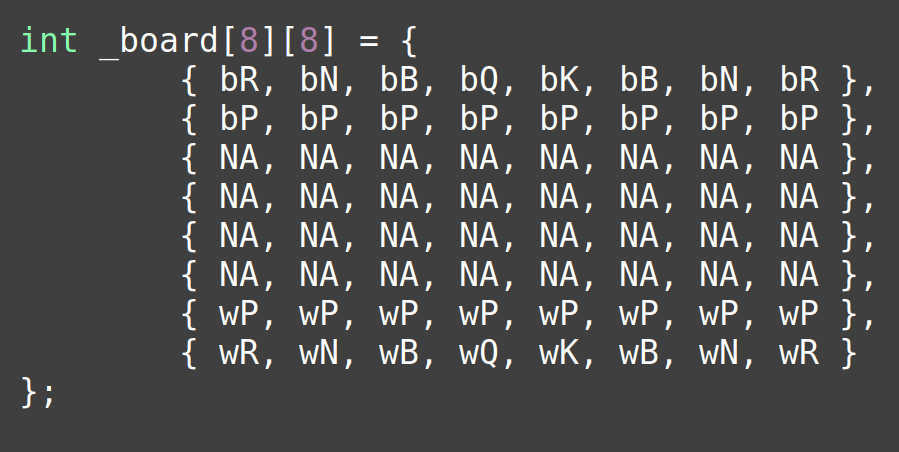
\includegraphics[width=0.8\textwidth]{board_representation.png} % Adjust the size as needed
        \caption{8 x 8 Array of Enums}
    \end{figure}
\end{frame}




\begin{frame}{Board Representation}
    \begin{figure}
        \centering
        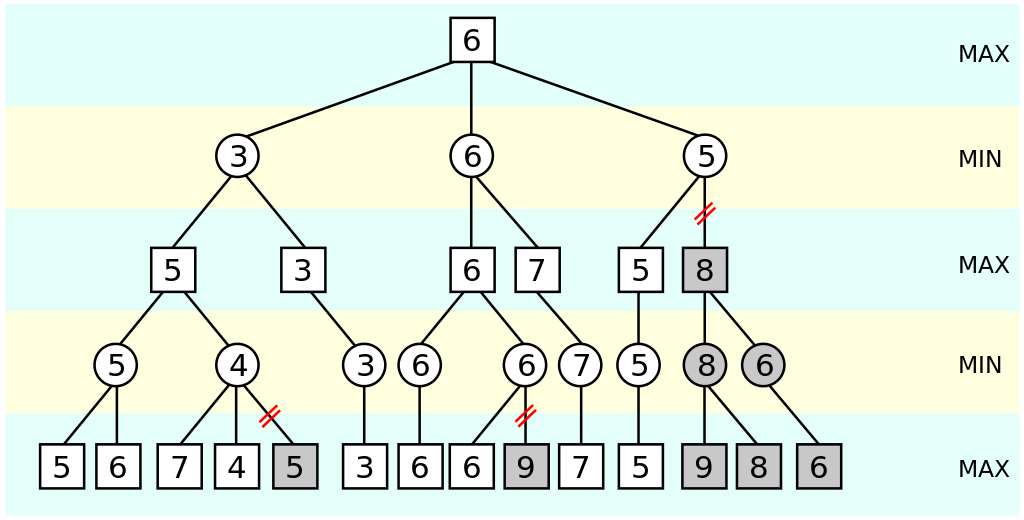
\includegraphics[width=0.8\textwidth]{minimax.png} % Adjust the size as needed

        \caption{8 x 8 Array of Enums}
    \end{figure}
\href{https://en.wikipedia.org/wiki/Alpha\%E2\%80\%93beta_pruning}{Wikipedia}
\end{frame}





\begin{frame}{Evaluation}
\begin{table}[ht]
\centering
\begin{tabular}{|l|c|}
\hline
\textbf{Chess Piece} & \textbf{Value} \\
\hline
Pawn & 1 \\
\hline
Knight & 3 \\
\hline
Bishop & 3 \\
\hline
Rook & 5 \\
\hline
Queen & 9 \\
\hline
King & 50 \\
\hline
\end{tabular}
\caption{Values assigned to each chess piece for evaluation.}
\label{table:chess_piece_values}
\end{table}
\end{frame}

\begin{frame}{It's Playable! (github.com/Aki78/ChessAI)}
    \begin{figure}
        \centering
        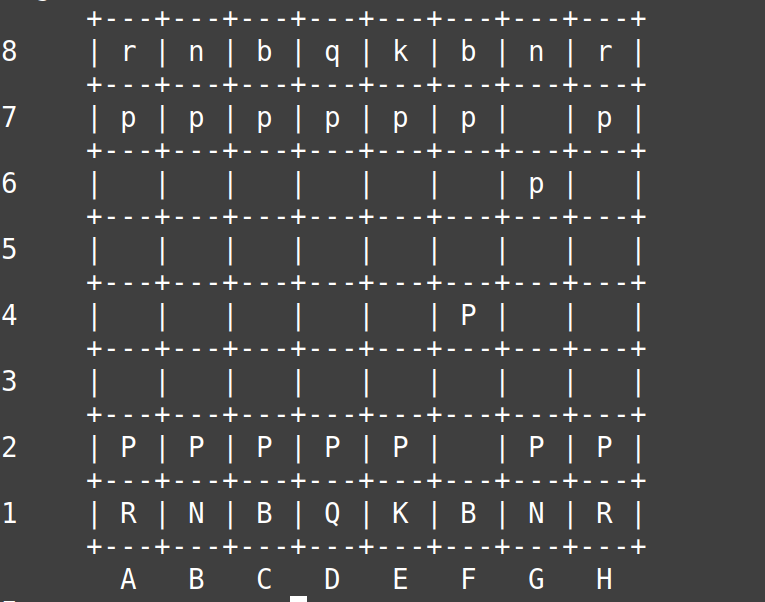
\includegraphics[width=0.7\textwidth]{playable.png} % Adjust the size as needed

    \end{figure}
\end{frame}


\begin{frame}{Against 1500 Elo AI (chess.com)}
    \begin{figure}
        \centering
        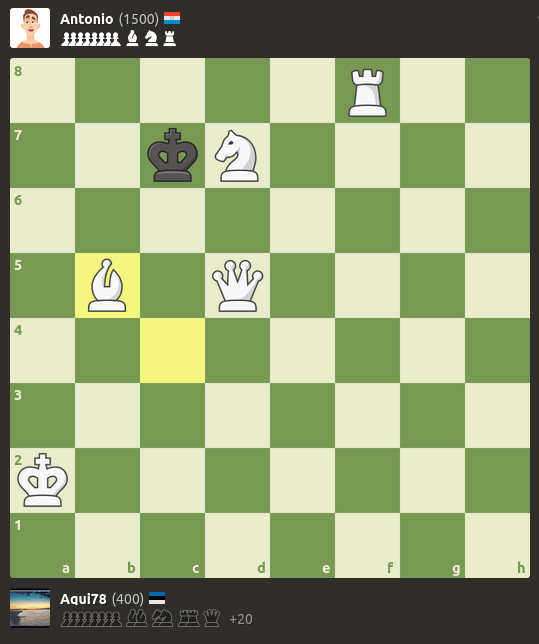
\includegraphics[width=0.4\textwidth]{play1500.png} % Adjust the size as needed
        \caption{Draw: easily took all pieces, but couldn't finish it. (depth = 5 )}

    \end{figure}
\end{frame}

%\begin{frame}{Comparative Images}
%  \begin{columns}[T] % The [T] option aligns column content at the top
%    \begin{column}{.48\textwidth} % Left column
%      \centering
%      
\includegraphics[width=0.8\linewidth]{logo.png} % Left image
%      \captionof{figure}{Caption here}
%    \end{column}
%    \begin{column}{.48\textwidth} % Right column
%      \centering
%      
\includegraphics[width=0.8\linewidth]{logo.png} % Right image
%      \captionof{figure}{Caption here}
%    \end{column}
%
%  \end{columns}
%\end{frame}

\section{Further Development}

\begin{frame}{Further Development}
  \begin{itemize}
    \item Better Evaluation Function
    \item Reordering Moves for $\alpha$ - $\beta$ pruning
    \item Using bit operations with a bit representation
    \item Use Opening books and End Game Tables
    \item Machine Learning? $\rightarrow$ Need a super computer
    \item etc. etc.
  \end{itemize}
\end{frame}


\end{document}

